\chapter{The Monte Carlo Random Walk Process for Adjoint Radiation Transport}
\label{ch:adjoint_particle_transport}
In section \ref{sec:dual_problems} the dual FIESK was introduced as a way to
estimate the value of interest, which for radiation transport problems is
defined in equation \ref{eq:material_response}, at a point. In this chapter the 
dual emission density FIESK will be shown. In addition, more general PDFs that 
govern the random walk process for adjoint radiation will be derived. The same 
steps that were outlined in the previous chapter will be followed to derive 
these PDFs.  

\section{The Dual Emission Density FIESK}
Using the procedure outlined in section \ref{sec:dual_problems}, the dual 
emission density FIESK will be constructed. The function that will solve this 
dual equation will be called the \textit{adjoint of the emission density}. It 
is not called the adjoint emission density because, as will be shown, the
\textit{adjoint of the emission density} does not behave like an emission 
density (or in general an event density). First, a linear operator will be 
constructed from equation \ref{eq:emission_density_integral_eqn}, which is the 
emission density FIESK:
\begin{equation}
  \begin{split}
    H_{\chi} \cdot &\chi(\vec{r},E,\hat{\Omega}) = 
    \chi(\vec{r},E,\hat{\Omega}) - \\
    & \int\int\int C(\vec{r},E^{'} \to E,\hat{\Omega}^{'} \to \hat{\Omega})
    T(\vec{r}^{'} \to \vec{r},E^{'},\hat{\Omega}^{'}) 
    \chi(\vec{r}^{'},E',\hat{\Omega}^{'}) dV^{'}dE^{'}E\hat{\Omega}^{'}.
  \end{split}
\end{equation}
With the operator $H_{\chi}$ defined in this way it is clear from equation
\ref{eq:emission_density_integral_eqn} that 
\begin{equation}
H_{\chi} \cdot \chi(\vec{r},E,\hat{\Omega}) = S(\vec{r},E,\hat{\Omega}).
\end{equation}

To define the adjoint operator, the following equality must hold: 
\begin{equation*}
  \langle \chi^{\dagger}H_{\chi} \cdot \chi \rangle = 
  \langle \chi H_{\chi}^{\dagger} \cdot \chi^{\dagger} \rangle.
\end{equation*}
The brackets indicate integration over all phase space. The function 
$\chi^{\dagger}(\vec{r},E,\hat{\Omega})$ is the 
\textit{adjoint of the emission density}. Since the operator $H_{\chi}$ is known,
the left bracket will be expanded:
\begin{align}
  \langle \chi^{\dagger}H_{\chi} \cdot \chi \rangle & =
  \int\int\int \
  \chi^{\dagger}(\vec{r},E,\hat{\Omega}) \chi(\vec{r},E,\hat{\Omega})
  dV dE d\hat{\Omega} - \int\int\int \chi^{\dagger}(\vec{r},E,\hat{\Omega}) 
  \nonumber \\
  \cdot \int\int\int 
  C(\vec{r}&,E^{'} \to E, \hat{\Omega}^{'} \to \hat{\Omega}^{'})
  T(\vec{r}^{'} \to \vec{r},E^{'},\hat{\Omega}^{'})
  \chi(\vec{r}^{'},E^{'},\hat{\Omega}^{'}) dV^{'}dE^{'}d\hat{\Omega}^{'}
  dV dE d\hat{\Omega} \nonumber \\
  & = \int\int\int \
  \chi^{\dagger}(\vec{r},E,\hat{\Omega}) \chi(\vec{r},E,\hat{\Omega})
  dV dE d\hat{\Omega} - \int\int\int \chi(\vec{r}^{'},E^{'},\hat{\Omega}^{'}) 
  \nonumber \\
  \cdot \int\int\int 
  C(\vec{r}&,E^{'} \to E, \hat{\Omega}^{'} \to \hat{\Omega}^{'})
  T(\vec{r}^{'} \to \vec{r},E^{'},\hat{\Omega}^{'})
  \chi^{\dagger}(\vec{r},E,\hat{\Omega}) dV dE d\hat{\Omega}
  dV^{'}dE^{'}d\hat{\Omega}^{'}. \nonumber
\end{align}
From this last manipulation, the adjoint operator can be deduced: 
\begin{equation}
  \begin{split}
    H_{\chi}^{\dagger} \cdot &\chi^{\dagger}(\vec{r},E,\hat{\Omega}) = 
    \chi^{\dagger}(\vec{r},E,\hat{\Omega}) - \\
    & \int\int\int T(\vec{r} \to \vec{r}^{'},E,\hat{\Omega}) 
    C(\vec{r}^{'},E \to E^{'},\hat{\Omega} \to \hat{\Omega}^{'})
    \chi(\vec{r}^{'},E',\hat{\Omega}^{'}) dE^{'}d\hat{\Omega}^{'}dV^{'}.
  \end{split}
\end{equation}

In the previous chapter, the function $c(\vec{r},E,\hat{\Omega})$ was defined 
in equation \ref{eq:emission_response_function}, which should be used with 
the emission density to calculate a response. By forcing the adjoint 
operator acting on the \textit{adjoint of the emission density} to equal the 
function $c(\vec{r},E,\hat{\Omega})$, the dual emission density FIESK can be 
created:
\begin{equation}
  \begin{split}
    \chi^{\dagger}(\vec{r},&E,\hat{\Omega}) = c(\vec{r},E,\hat{\Omega}) + \\
    &\int\int\int T(\vec{r} \to \vec{r}^{'},E,\hat{\Omega}) 
    C(\vec{r}^{'},E \to E^{'},\hat{\Omega} \to \hat{\Omega}^{'})
    \chi^{\dagger}(\vec{r}^{'},E',\hat{\Omega}^{'}) dE^{'}d\hat{\Omega}^{'}dV^{'}.
  \end{split}
  \label{eq:adjoint_of_emission_density_integral_eqn}
\end{equation}

Unfortunately, in the integral in equation 
\ref{eq:adjoint_of_emission_density_integral_eqn}, the transport and collision 
kernels are integrated over what were previously the final states. Therefore,
the properties that were defined for these kernels in the previous chapter are 
no longer valid. In particular, the transport kernel is not normalized anymore
and the collision kernel does not integrate to the the average number of 
particles emitted from a collision. To renormalize these kernels, the 
$\Sigma_T(\vec{r}^{'},E)$ terms in both the transport and collision kernels will
be allowed to cancel each other out. The modified transport kernel will now be 
examined:
\begin{equation}
  \frac{T(\vec{r} \to \vec{r}^{'},E,\hat{\Omega})}{\Sigma_T(\vec{r}^{'},E)} = 
  \exp{\left[-\int_0^{|\vec{r}^{'} - \vec{r}|} 
    \Sigma_T(\vec{r}^{'} - R^{'} \hat{\Omega},E)dR^{'} \right]}
  \frac{\delta \left(\Omega - \left[\frac{\vec{r}^{'} - \vec{r}}
      {|\vec{r}^{'} - \vec{r}|}\right]\right)}
       {|\vec{r}^{'} - \vec{r}|^2}.
  \label{eq:unnormalized_adjoint_transport_kernel}
\end{equation}
Based on the argument of the delta function, 
\begin{align}
  \hat{\Omega} & = \frac{\vec{r}^{'} - \vec{r}}{|\vec{r}^{'} - \vec{r}|} 
  \nonumber \\
  & \text{ and} \nonumber \\
  \vec{r}^{'} & = \vec{r} + \hat{\Omega}|\vec{r}^{'} - \vec{r}|.
\end{align}
This equation for $\vec{r}^{'}$ can be substituted back into the equation
\ref{eq:unnormalized_adjoint_transport_kernel}:
\begin{equation*}
  \frac{T(\vec{r} \to \vec{r}^{'},E,\hat{\Omega})}{\Sigma_T(\vec{r}^{'},E)} = 
  \exp{\left[-\int_0^{|\vec{r}^{'} - \vec{r}|} 
    \Sigma_T \left(\vec{r} + \left[|\vec{r}^{'} - \vec{r}| - R^{'} \right]
    \hat{\Omega},E \right) dR^{'} 
    \right]} \frac{\delta \left(\Omega - \left[\frac{\vec{r}^{'} - \vec{r}}
      {|\vec{r}^{'} - \vec{r}|}\right]\right)}
       {|\vec{r}^{'} - \vec{r}|^2}.
\end{equation*}
A new variable of integration can be defined to simplify the exponent:
\begin{align}
  R^{''} & = |\vec{r}^{'} - \vec{r}| - R^{'} \\
  dR^{''} & = -dR^{'} \nonumber 
\end{align}
Note that $R^{''} = 0$ when $R^{'} = |\vec{r}^{'} - \vec{r}|$ and 
$R^{''} = |\vec{r}^{'} - \vec{r}|$ when $R^{'} = 0$. Equation 
\ref{eq:unnormalized_adjoint_transport_kernel} now becomes
\begin{align}
  \frac{T(\vec{r} \to \vec{r}^{'},E,\hat{\Omega})}{\Sigma_T(\vec{r}^{'},E)} & =
  \exp{\left[-\int_0^{|\vec{r}^{'} - \vec{r}|} 
    \Sigma_T \left(\vec{r} + R^{''}\hat{\Omega},E \right) dR^{''} 
    \right]} \frac{\delta \left(\Omega - \left[\frac{\vec{r}^{'} - \vec{r}}
      {|\vec{r}^{'} - \vec{r}|}\right]\right)}
       {|\vec{r}^{'} - \vec{r}|^2} \nonumber \\
       & = \exp{\left[-\int_0^{|\vec{r} - \vec{r}^{'}|} 
    \Sigma_T \left(\vec{r} + R^{''}\hat{\Omega},E \right) dR^{''} 
    \right]} \frac{\delta \left(\Omega + \left[\frac{\vec{r} - \vec{r}^{'}}
      {|\vec{r} - \vec{r}^{'}|}\right]\right)}
       {|\vec{r} - \vec{r}^{'}|^2} \nonumber \\
       & = \tau(\vec{r}^{'},\vec{r},E,-\hat{\Omega}) \\
       & = \frac{T(\vec{r}^{'} \to \vec{r},E,-\hat{\Omega})}
       {\Sigma_T(\vec{r},E)}.
\end{align}
The dual emission density FIESK is therefore
\begin{equation}
  \chi^{\dagger}(\vec{r},E,\hat{\Omega}) =  c(\vec{r},E,\hat{\Omega}) +
  \int\int\int  \tau(\vec{r}^{'},\vec{r},E,-\hat{\Omega}) 
  \Sigma_T(\vec{r}^{'},E \to E^{'},\hat{\Omega} \to \hat{\Omega}^{'})
  dE^{'}d\hat{\Omega}^{'}dV^{'}.
  \label{eq:adjoint_of_emission_density_integral_eqn_2}
\end{equation}
 
By comparing equation \ref{eq:adjoint_of_emission_density_integral_eqn_2} to 
the flux FIESK given in equation \ref{eq:flux_integral_equation}, it is clear 
that the \textit{adjoint of the emission density} behaves very similar to the 
flux. In the literature, the \textit{adjoint of the emission density} is often 
called ``flux-like'' because of this similarity \citep{hoogenboom_adjoint_1977}.
Though it will not be shown, the \textit{adjoint of the collision density} is 
also ``flux-like.'' In section \ref{sec:flux_fiesk} it was shown that the random
walk process to estimate the flux was not ideal. While a random walk process 
could be constructed for the \textit{adjoint of the emission density}, given its
flux-like nature, its random walk process will not be ideal either. 

One way to construct a function that will be collision like and still retain
the desired property of the dual FIESK (i.e. the response function 
becomes the source) is to multiply equation 
\ref{eq:adjoint_of_emission_density_integral_eqn_2} by some function 
$\Sigma^{*}(\vec{r},E)$, whose only necessary properties are that it is
strictly positive and that it goes to zero in a vacuum. While this manipulation
is encountered in several pieces of literature, and is in fact necessary in
the derivation of the probability laws for coupled adjoint neutron and adjoint 
photon transport, it will be more instructive to take a step back and start over
again with the adjoint transport equation 
\citep{kalos_monte_1968, eriksson_monte_1969, hoogenboom_methodology_2003}. In 
addition, the process for deriving the PDFs that govern the random walk process 
for the emission density and collision density outlined in the previous chapter 
can be followed. 

\section{The Adjoint Integro-Differential Boltzmann Equation}
The integro-differential transport equation, given in equation 
\ref{eq:integro_diff_boltzmann_eqn} can also be written in an operator form. 
In the following equation, it is assumed that the flux distribution is 
time-independent:
\begin{equation}
  H_B \cdot \varphi(\vec{r},E,\hat{\Omega}) = S(\vec{r},E,\hat{\Omega}).
\end{equation}
Using the integro-differential transport operator, and the following
equality
\begin{equation}
  \langle \varphi^{\dagger}H_B \cdot \varphi \rangle = 
  \langle \varphi H_B^{\dagger} \cdot \varphi^{\dagger} \rangle,
\end{equation}
the adjoint integro-differential transport operator can be derived
\citep{lewis_computational_1993, bell_nuclear_1979}. This derivation is quite 
lengthy and will therefore not be shown. The interested reader should refer to 
the text by Lewis and Miller or the text by Bell and Glasstone for this 
derivation \citep{lewis_computational_1993, bell_nuclear_1979}. The function 
$\varphi^{\dagger}(\vec{r},E,\hat{\Omega})$ is the adjoint flux. The adjoint
integro-differential transport operator, which operates on the adjoint flux,
is
\begin{equation}
  \begin{split}
    H_B^{\dagger} \cdot \varphi^{\dagger}(\vec{r},E,\hat{\Omega}) &= 
    \left[ -\hat{\Omega} \cdot \vec{\bigtriangledown} +
     \Sigma_T(\vec{r},E) \right] \varphi^{\dagger}(\vec{r},E,\hat{\Omega}) - \\
     & \int\int \Sigma_T(\vec{r},E \to E^{'},\hat{\Omega} \to \hat{\Omega}^{'})
    \varphi^{\dagger}(\vec{r},E^{'},\hat{\Omega}^{'}) dE^{'} d\hat{\Omega}^{'}.
  \end{split}
  \label{eq:integro_diff_adj_trans_op}
\end{equation}

The adjoint integro-differential transport equation can be derived by
forcing $H_B^{\dagger} \cdot \varphi^{\dagger}(\vec{r},E,\hat{\Omega})$ to equal
the response function $a(\vec{r},E,\hat{\Omega})$ that was used in equation
\ref{eq:material_response}. This will ensure that the inner product of the 
adjoint flux and the source will give the same value as the inner product of 
the flux and the response function:
\begin{align}
  I & = \langle \varphi H_B^{\dagger} \cdot \varphi^{\dagger} \rangle \nonumber \\
  & = \langle \varphi a \rangle \nonumber \\
  & = \langle \varphi^{\dagger}H_B \cdot \varphi \rangle \nonumber \\
  & = \langle \varphi^{\dagger} S \rangle \nonumber.
\end{align}
The adjoint integro-differential transport equation is 
\begin{equation}
  \begin{split}
    -\hat{\Omega} &\cdot \vec{\bigtriangledown} 
    \varphi^{\dagger}(\vec{r},E,\hat{\Omega})
    + \Sigma_T(\vec{r},E) \varphi^{\dagger}(\vec{r},E,\hat{\Omega}) = \\
    & \quad a(\vec{r},E,\hat{\Omega}) +
    \int\int \Sigma_T(\vec{r},E \to E^{'},\hat{\Omega} \to \hat{\Omega}^{'})
    \varphi^{\dagger}(\vec{r},E^{'},\hat{\Omega}^{'}) dE^{'}d\hat{\Omega}^{'}.
  \end{split}
  \label{eq:integro_diff_adj_boltzmann_eqn}
\end{equation}

It must be noted that the double differential collision cross section in the
adjoint integro-differential transport equation is identical to the one that
appears in the integro-differential transport equation. However, it is now
integrated over final energies and directions. Therefore, it is not clear what 
the normalization for the total double differential transfer function is or 
equivalently, what the mean number of adjoint particles emerging per collision 
is. These properties of the total double differential transfer function will
be analyzed in the coming sections.

\section{The Adjoint Transport Equation in Integral Form}
In order to use the Monte Carlo random walk process that was discussed
in the chapter \ref{ch:mc_methods}, the integro-differential form of the adjoint
transport equation must be converted to a FIESK. To do this, the adjoint
transport equation will first be simplified by introducing the adjoint emission
density: 
\begin{equation}
  \theta^{\dagger}(\vec{r},E,\hat{\Omega}) = a(\vec{r},E,\hat{\Omega}) +
  \int\int \Sigma_T(\vec{r},E \to E^{'},\hat{\Omega} \to \hat{\Omega}^{'})
  \varphi^{\dagger}(\vec{r},E^{'},\hat{\Omega}^{'}) dE^{'}d\hat{\Omega}^{'}.
  \label{eq:adjoint_emission_density}
\end{equation}
The adjoint emission density is the expected density of adjoint particles 
exiting a collision or the adjoint source. Using this definition for the
adjoint emission density, the simplified adjoint transport equation becomes
\begin{equation}
  -\hat{\Omega} \cdot \vec{\bigtriangledown} 
    \varphi^{\dagger}(\vec{r},E,\hat{\Omega},t)
    + \Sigma_T(\vec{r},E) \varphi^{\dagger}(\vec{r},E,\hat{\Omega},t) =
    \theta^{\dagger}(\vec{r},E,\hat{\Omega}).
\end{equation}
  
From the reduced adjoint transport equation, the method of characteristics will
be used to transform it to its integral form. The characteristic for the 
adjoint transport equation is the following parameterized line.
\begin{equation}
  \vec{r}^{'} = \vec{r} + R\hat{\Omega}
  \label{eq:adjoint_characteristic}
\end{equation}
Using equation \ref{eq:adjoint_characteristic} a directional derivative along
the characteristic can be determined:
\begin{align}
  \frac{d}{dR} & = \frac{dx^{'}}{dR}\frac{\partial}{\partial x} +
  \frac{dy^{'}}{dR}\frac{\partial}{\partial y} +
  \frac{dz^{'}}{dR}\frac{\partial}{\partial z} \nonumber \\
  & = \Omega_x \frac{\partial}{\partial x} +
  \Omega_y \frac{\partial}{\partial y} +
  \Omega_z \frac{\partial}{\partial z} \nonumber \\
  & = \hat{\Omega} \cdot \vec{\bigtriangledown}.
\end{align}
By using the directional derivative along the characteristic the adjoint 
transport equation can be reduced to a first order ODE:
\begin{equation}
  -\frac{d}{dR}\varphi^{\dagger}(\vec{r}^{'},E,\hat{\Omega}) + 
  \Sigma_T(\vec{r}^{'},E)
  \varphi^{\dagger}(\vec{r}^{'},E,\hat{\Omega}) = 
  \theta^{\dagger}(\vec{r}^{'},E,\hat{\Omega}).
  \label{eq:adjoint_transport_ode}
\end{equation}
This ODE can be easily solved with the integrating factor
\begin{equation} 
  \exp{\left[-\int_0^R \Sigma_T(\vec{r}+R^{'}\hat{\Omega},E)dR^{'} \right]},
\end{equation}
as will be shown.

First, the left two terms of equation \ref{eq:adjoint_transport_ode} can
combined into a single term using the integrating factor:
\begin{align}
  -\frac{d}{dR}\bigg[\varphi^{\dagger}(\vec{r}^{'},E,\hat{\Omega})
    \exp{\left[-\int_0^R \Sigma_T(\vec{r}+R^{'}\hat{\Omega},E)dR^{'}\right]}
    \bigg] = \nonumber \\
  \theta^{\dagger}(\vec{r}^{'},E,\hat{\Omega})
  &\exp{\left[-\int_0^R \Sigma_T(\vec{r}+R^{'}\hat{\Omega},E)dR^{'} \right]}.
  \nonumber
\end{align}
Next, the derivative along the characteristic can be eliminated by integrating
from zero to infinity:
\begin{align}
  -\varphi^{\dagger}(\vec{r} + R\hat{\Omega},E,\hat{\Omega})
  \exp{\left[-\int_0^R \Sigma_T(\vec{r}+R^{'}\hat{\Omega},E)dR^{'}\right]}
  \bigg|_0^{\infty} & = \nonumber \\
  \int_0^{\infty} 
  \theta^{\dagger}(\vec{r} + R\hat{\Omega},E,\hat{\Omega})
  &\exp{\left[-\int_0^R \Sigma_T(\vec{r}+R^{'}\hat{\Omega},E)dR^{'} \right]} dR.
  \nonumber 
\end{align}
If the adjoint flux is assumed to go to zero as R goes to infinity, the integral
adjoint transport equation is obtained:
\begin{equation}
  \varphi^{\dagger}(\vec{r},E,\hat{\Omega}) = 
  \int_0^{\infty} \theta^{\dagger}(\vec{r} + R\hat{\Omega},E,\hat{\Omega})
  exp\left[-\int_0^R \Sigma_T(\vec{r}+R^{'}\hat{\Omega},E)dR^{'} \right] dR.
  \label{eq:line_integral_adj_transport_eqn}
\end{equation}

Like with the integral transport equation, it is often more convenient to 
represent the integral adjoint transport equation as an integral over all space.
To do this, note that
\begin{align}
  R & = |\vec{r}^{'} - \vec{r}|, \nonumber \\
  \hat{\Omega} & = \frac{\vec{r}^{'} - \vec{r}}{|\vec{r}^{'} - \vec{r}}| 
  \text{ and} \nonumber \\
  dV^{'} & = R^2dRd\hat{\Omega}. \nonumber \\
\end{align}
With these definitions, the integral adjoint transport equation becomes
\begin{equation*}
    \varphi^{\dagger}(\vec{r},E,\hat{\Omega}) = 
    \int \theta^{\dagger}(\vec{r}^{'},E,\hat{\Omega})
    \exp{\left[-\int_0^{|\vec{r}^{'} - \vec{r}|} 
      \Sigma_T(\vec{r}+R^{'}\hat{\Omega},E)dR^{'} \right]}
    \frac{\delta \left(\Omega - \left[\frac{\vec{r}^{'} - \vec{r}}
        {|\vec{r}^{'} - \vec{r}|}\right]\right)}
    {|\vec{r}^{'} - \vec{r}|^2} dV^{'}.
\end{equation*}

To further simplify the integral adjoint transport equation, one more function
will be introduced:
\begin{equation}
  \tau^{\dagger}(\vec{r}^{'},\vec{r},E,\hat{\Omega}) = 
  \exp{\left[-\int_0^{|\vec{r}^{'} - \vec{r}|} 
      \Sigma_T(\vec{r}+R^{'}\hat{\Omega},E)dR^{'} \right]}
    \frac{\delta \left(\Omega - \left[\frac{\vec{r}^{'} - \vec{r}}
        {|\vec{r}^{'} - \vec{r}|}\right]\right)}
    {|\vec{r}^{'} - \vec{r}|^2}.
\end{equation}
By inspection it is clear that this function is simply the function 
introduced in equation \ref{eq:unnormalized_transport_kernel} with a negative
angular variable:
\begin{equation}
  \tau^{\dagger}(\vec{r}^{'},\vec{r},E,\hat{\Omega}) = 
  \tau(\vec{r}^{'},\vec{r},E,-\hat{\Omega}).
\end{equation}
The simplified integral adjoint transport equation is now simply
\begin{equation}
  \varphi^{\dagger}(\vec{r},E,\hat{\Omega}) = 
    \int \theta^{\dagger}(\vec{r}^{'},E,\hat{\Omega}) 
    \tau^{\dagger}(\vec{r}^{'},\vec{r},E,\hat{\Omega}) dV^{'}.
  \label{eq:volume_integral_adj_transport_eqn}
\end{equation}

Based on the lessons that were learned in the previous chapter, the adjoint
flux FIESK will not be created and instead, the adjoint emission density FIESK 
will be derived next.

\section{The Adjoint Emission Density FIESK}
To construct the adjoint emission density FIESK the integral adjoint transport
equation given in equation \ref{eq:volume_integral_adj_transport_eqn} must be 
substituted back into the adjoint emission density shown in equation 
\ref{eq:adjoint_emission_density}:
\begin{align}
  \theta^{\dagger}(\vec{r},E,\hat{\Omega}) & = a(\vec{r},E,\hat{\Omega}) +
  \int\int \Sigma_T(\vec{r},E \to E^{'},\hat{\Omega} \to \hat{\Omega}^{'})
  \int \theta^{\dagger}(\vec{r}^{'},E^{'},\hat{\Omega}^{'}) 
  \tau^{\dagger}(\vec{r}^{'},\vec{r},E^{'},\hat{\Omega}^{'}) 
  dV^{'} dE^{'} d\hat{\Omega}^{'} \nonumber \\
  & = a(\vec{r},E,\hat{\Omega}) +
  \int\int\int \frac{\Sigma^{\dagger}(\vec{r},E^{'})}{\Sigma_T(\vec{r},E^{'})}
  \frac{\Sigma_T(\vec{r},E \to E^{'},\hat{\Omega} \to \hat{\Omega}^{'})}
       {\Sigma^{\dagger}(\vec{r},E^{'})} \Sigma_T(\vec{r},E^{'})
  \tau^{\dagger}(\vec{r}^{'},\vec{r},E^{'},\hat{\Omega}^{'}) \nonumber \\
  & \qquad \qquad \qquad \qquad \qquad \cdot
  \theta^{\dagger}(\vec{r}^{'},E^{'},\hat{\Omega}^{'}) 
  dV^{'} dE^{'} d\hat{\Omega}^{'}. \nonumber
\end{align}
The function $\Sigma^{\dagger}(\vec{r},E^{'})$ is called the total macroscopic
adjoint cross section and is defined as
\begin{equation}
  \Sigma^{\dagger}(\vec{r},E^{'}) = \int\int 
  \Sigma_T(\vec{r},E \to E^{'},\hat{\Omega} \to \hat{\Omega}^{'}) 
  dEd\hat{\Omega}.
  \label{eq:total_adjoint_cross_section}
\end{equation}

Two kernels and one weight factor must now be introduced to simplify
the adjoint emission density FIESK. The first kernel will be called the 
adjoint collision kernel and is defined as
\begin{align}
  C^{\dagger}(\vec{r},E^{'} \to E,\hat{\Omega}^{'} \to \hat{\Omega}) & = 
  \frac{\Sigma_T(\vec{r},E \to E^{'},\hat{\Omega} \to \hat{\Omega}^{'})}
  {\int\int \Sigma_T(\vec{r},E \to E^{'},\hat{\Omega} \to \hat{\Omega}^{'})
    dE d\hat{\Omega}} \nonumber \\
  & = \frac{\Sigma_T(\vec{r},E \to E^{'},\hat{\Omega} \to \hat{\Omega}^{'})}
           {\Sigma^{\dagger}(\vec{r},E^{'})}.
  \label{eq:adj_collision_kernel}
\end{align}
The second kernel will be called the adjoint transport kernel and is defined as
\begin{align}
  T^{\dagger}(\vec{r}^{'} \to \vec{r},E,\hat{\Omega}) & = 
  \Sigma_T(\vec{r},E) \tau^{\dagger}(\vec{r}^{'},\vec{r},E,\hat{\Omega})
  \nonumber \\
  & = \Sigma_T(\vec{r},E) \exp{\left[-\int_0^{|\vec{r}^{'} - \vec{r}|} 
      \Sigma_T(\vec{r}+R^{'}\hat{\Omega},E)dR^{'} \right]}
    \frac{\delta \left(\Omega - \left[\frac{\vec{r}^{'} - \vec{r}}
        {|\vec{r}^{'} - \vec{r}|}\right]\right)}
    {|\vec{r}^{'} - \vec{r}|^2}.
\end{align}
The quantity $T^{\dagger}(\vec{r}^{'} \to \vec{r},E,\hat{\Omega})dV$ can be
interpreted as the probability that an adjoint particle at $\vec{r}^{'}$ with
energy $E$ and direction $\hat{\Omega}$ will have its next collision in volume
element $dV$ at $\vec{r}$.

The weight factor will be called the adjoint weight factor. It is defined as
\begin{equation}
  P^{\dagger}(\vec{r},E) = \frac{\Sigma^{\dagger}(\vec{r},E)}
  {\Sigma_T(\vec{r},E)}.
\end{equation}
The adjoint weight factor comes about from the construction of the adjoint
collision kernel and the adjoint transport kernel. To construct the adjoint
collision kernel from the double differential collision cross section, one
must divide the double differential collision cross section by the total
macroscopic adjoint cross section. To construct the adjoint transport kernel
one must multiply the function 
$\tau^{\dagger}(\vec{r}^{'},\vec{r},E,\hat{\Omega})$ by the total macroscopic
cross section. In general, the total macroscopic adjoint cross section
and the total macroscopic cross section will not be equal, which is why the
adjoint weight factor arises. In some literature, this factor is called 
the adjoint non-absorption probability \citep{gabler_amos_2006}. However, as 
will be shown in the next chapter, this factor is not bounded in the 
interval (0,1) but is instead bounded in the interval (0,$\infty$). It is 
therefore inappropriate to call this factor a probability\footnote{This fact is
noted in the reference that calls the factor the adjoint non-absorption 
probability \citep{gabler_amos_2006}.}.

Using the above kernels and weight factor, the simplified adjoint emission
density FIESK becomes
\begin{equation}
  \begin{split}
    \theta^{\dagger}(\vec{r},E,\hat{\Omega}) = a(\vec{r},E,\hat{\Omega}) + 
    \int\int&\int 
    C^{\dagger}(\vec{r},E^{'} \to E,\hat{\Omega}^{'} \to \hat{\Omega}) 
    P^{\dagger}(\vec{r},E^{'}) \\
    & \cdot T^{\dagger}(\vec{r}^{'} \to \vec{r},E^{'},\hat{\Omega}^{'})
    \theta^{\dagger}(\vec{r}^{'},E^{'},\hat{\Omega}^{'})
    dV^{'} dE^{'} d\hat{\Omega}^{'}.
  \end{split}
  \label{eq:adj_emission_dens_int_eqn}
\end{equation}

The state transition kernel for the adjoint emission density FIESK is simply
\begin{align}
  M^{\dagger}(y \to x) & = 
  M^{\dagger}(\vec{r}^{'} \to \vec{r},E^{'} \to E,\hat{\Omega}^{'} \to \hat{\Omega})
  \nonumber \\
  & = C^{\dagger}(\vec{r},E^{'} \to E,\hat{\Omega}^{'} \to \hat{\Omega})
  P^{\dagger}(\vec{r},E^{'})
  T^{\dagger}(\vec{r}^{'} \to \vec{r},E^{'},\hat{\Omega}^{'}).
  \label{eq:adj_emission_dens_kernel}
\end{align}

\section{The Adjoint Collision Density FIESK}
Like the collision density, the adjoint collision density can also be quite
useful. It is related to the adjoint flux and the adjoint emission density by 
the following equations, which are analogous to the relationships between the 
collision density, flux and emission density:
\begin{align}
  \xi^{\dagger}(\vec{r},E,\hat{\Omega}) & = \Sigma_T(\vec{r},E)
  \varphi^{\dagger}(\vec{r},E,\hat{\Omega}) \\
  & = \int T^{\dagger}(\vec{r}^{'} \to \vec{r},E,\hat{\Omega})
  \theta^{\dagger}(\vec{r}^{'},E,\hat{\Omega}) dV^{'}.
  \label{eq:adj_collision_dens_to_adj_emission_dens}
\end{align}
The adjoint collision density is the density of adjoint particles entering a 
collision. 

To construct the adjoint collision density FIESK, equation 
\ref{eq:adj_collision_dens_to_adj_emission_dens} and the adjoint emission
density FIESK given in equation \ref{eq:adj_emission_dens_int_eqn} will be
used:
\begin{align}
  \xi^{\dagger}(\vec{r},E,\hat{\Omega}) & = \int a(\vec{r}^{'},E,\hat{\Omega})
  T^{\dagger}(\vec{r}^{'} \to \vec{r},E,\hat{\Omega}) dV^{'} + \nonumber \\
  &\quad \int\int\int T^{\dagger}(\vec{r}^{'} \to \vec{r},E,\hat{\Omega})
  C^{\dagger}(\vec{r}^{'},E^{'} \to E, \hat{\Omega}^{'} \to \hat{\Omega})
  P^{\dagger}(\vec{r}^{'},E^{'}) \xi^{\dagger}(\vec{r}^{'},E^{'},\hat{\Omega}^{'})
  dE^{'}d\hat{\Omega}^{'}dV^{'}.
  \label{eq:adj_collision_dens_int_eqn}
\end{align}
Notice that the source term for the adjoint collision density is a first
collided source. To avoid confusion with the source term for the collision
density, it will be referred to as the adjoint first collided source.

The state transition kernel for the collision density FIESK is simply
\begin{align}
  N^{\dagger}(y \to x) & =
  N^{\dagger}(\vec{r}^{'} \to \vec{r},E^{'} \to E,\hat{\Omega}^{'} \to \hat{\Omega})
  \nonumber \\
  & = T^{\dagger}(\vec{r}^{'} \to \vec{r},E,\hat{\Omega})
  C^{\dagger}(\vec{r}^{'},E^{'} \to E,\hat{\Omega}^{'} \to \hat{\Omega})
  P^{\dagger}(\vec{r}^{'},E^{'}).
\end{align}

\section{Adjoint Emission and Collision Density State Transition Kernel Properties}
Before the PDFs that govern the random walk process are derived, the adjoint
transport kernel, adjoint collision kernel and adjoint weight factor must be 
investigated a bit further. A comparison of the adjoint transport kernel and 
the transport kernel reveals that the adjoint transport kernel is identical 
the the transport kernel with $\hat{\Omega} = -\hat{\Omega}$:
\begin{equation}
  T^{\dagger}(\vec{r}^{'} \to \vec{r},E,\hat{\Omega}) = 
  T(\vec{r}^{'} \to \vec{r},E,-\hat{\Omega}).
\end{equation}
The significance of this relationship is that adjoint particles move in the 
direction opposite of the variable $\hat{\Omega}$. It is therefore 
inappropriate to interpret the variable $\hat{\Omega}$ of an adjoint particle 
as its direction. However, for convenience, it will continue to be referred to 
as an adjoint particle's direction. This relationship also indicates that the 
adjoint transport kernel is normalized for an infinite medium:
\begin{equation}
  \int T^{\dagger}(\vec{r}^{'} \to \vec{r},E,\hat{\Omega}) dV = 1.
\end{equation}
In problems where the domain of interest in finite, random walks should be 
terminated when they exit the domain of interest. This procedure was described
in the previous chapter to account for the unnormalized transport kernel in
finite domains. Because of the relationship between the transport kernel and 
the adjoint transport kernel, this procedure is also valid for the adjoint
transport kernel. 

Based on the definition of the adjoint collision kernel from equation
\ref{eq:adj_collision_kernel} the adjoint collision kernel is also normalized 
to unity:
\begin{align}
  \int\int C^{\dagger}(\vec{r},E^{'} \to E,\hat{\Omega}^{'} \to \hat{\Omega})
  dE d\hat{\Omega} & = \int\int 
  \frac{\Sigma_T(\vec{r},E \to E^{'},\hat{\Omega} \to \hat{\Omega}^{'})} 
       {\Sigma^{\dagger}(\vec{r},E^{'})} dEd\hat{\Omega} \nonumber \\
  & = 1. \nonumber 
\end{align}
This property of the adjoint collision kernel hints at two interesting
phenomena for adjoint particles. First, there are no absorption reactions for
adjoint particles and second, there are no multiplying reactions for adjoint
particles. Both of these properties become more obvious when the adjoint
collision is expanded, which will be done in the next section. The consequence 
of the lack of an adjoint absorption reaction is that an analogue random walk 
process for the adjoint FIESKs is not possible. Russian roulette will have to 
be used to terminate histories.

As mentioned before, the adjoint weight factor $P^{\dagger}(\vec{r},E)$ takes 
into account the fact that the total macroscopic cross section 
$\Sigma_T(\vec{r},E)$, which is used to construct the adjoint transport kernel, 
is not equal to the total macroscopic adjoint cross section  
$\Sigma^{\dagger}(\vec{r},E)$, which is used to construct the adjoint collision 
kernel. Unfortunately, this factor is not bounded to the interval (0,1), which 
means that it is likely to increase the variance of the estimators used. 

Based on the properties of the adjoint transport kernel, adjoint collision
kernel and the adjoint weight factor, the adjoint emission density state 
transition kernel normalization can be determined:
\begin{align}
  \int M^{\dagger}(y \to x)dx & = \int\int\int 
  C^{\dagger}(\vec{r},E^{'} \to E,\hat{\Omega}^{'} \to \hat{\Omega})
  P^{\dagger}(\vec{r},E^{'}) 
  T^{\dagger}(\vec{r}^{'} \to \vec{r},E^{'},\hat{\Omega}^{'}) dE d\hat{\Omega}) dV
  \nonumber \\
  & = \int P^{\dagger}(\vec{r},E^{'})
  T^{\dagger}(\vec{r}^{'} \to \vec{r},E^{'},\hat{\Omega}^{'}) dE d\hat{\Omega}) dV
  \nonumber \\
  & = \overline{P}^{\dagger}(\vec{r}^{'},E^{'}).
\end{align}
The normalization function $\overline{P}^{\dagger}(\vec{r}^{'},E^{'})$ can be
interpreted as the average adjoint weight factor along the line from
$\vec{r}^{'}$ to $\vec{r}$ given an adjoint particle of energy $E^{'}$.

The adjoint collision density state transition kernel normalization can also be
determined with the properties of the adjoint transport kernel, adjoint
collision kernel and adjoint weight factor that were discussed:
\begin{align}
  \int N^{\dagger}(y \to x)dx & = \int\int\int
  T^{\dagger}(\vec{r}^{'} \to \vec{r},E,\hat{\Omega})
  C^{\dagger}(\vec{r}^{'},E^{'} \to E,\hat{\Omega}^{'} \to \hat{\Omega})
  P^{\dagger}(\vec{r}^{'},E^{'}) dV dE d\hat{\Omega}) 
  \nonumber \\
  & = \int C^{\dagger}(\vec{r}^{'},E^{'} \to E,\hat{\Omega}^{'} \to \hat{\Omega})
  P^{\dagger}(\vec{r}^{'},E^{'}) dE d\hat{\Omega})
  \nonumber \\
  & = P^{\dagger}(\vec{r}^{'},E^{'}).
\end{align}

The properties of the two state transition kernels are summarized below. 
\begin{enumerate}
  \item $M^{\dagger}(y \to x) > 0$ \\
    $N^{\dagger}(y \to x) > 0$ \\ \\
    and
  \item $\int M^{\dagger}(y \to x)dx = \overline{P}^{\dagger}(y) < \infty$ \\
    $\int N^{\dagger}(y \to x)dx = P^{\dagger}(y) < \infty$
\end{enumerate}

Based on these properties for the two kernels and the fact that the adjoint
survival probability is always unity due to the lack of an absorption reaction,
it is clear that an analogue random walk process for adjoint radiation 
transport is impossible. The adjoint collision kernel must still be 
expanded into its constituent parts, which will be shown in the next section, 
so that each individual adjoint reaction can be treated explicitly. 

\section{Expansion of the Adjoint Collision Kernel}
As explained in the previous chapter, the total double differential transfer 
function, which appears in both the collision kernel and the adjoint collision 
kernel, is challenging to obtain. To conduct the random walks for adjoint 
radiation, each individual adjoint reaction has to be modeled. To do this, the 
adjoint collision kernel must be expanded:
\begin{align}
  C^{\dagger}(\vec{r},E^{'} \to E,\hat{\Omega}^{'} \to \hat{\Omega}) & =
  \frac{\Sigma_T(\vec{r},E \to E^{'},\hat{\Omega} \to \hat{\Omega}^{'})}
       {\Sigma^{\dagger}(\vec{r},E^{'})} \nonumber \\
       & = \sum_j 
       \frac{\Sigma_{j}(\vec{r},E)c_j(\vec{r},E)
         f_j(E \to E^{'},\hat{\Omega} \to \hat{\Omega}^{'})}
            {\Sigma^{\dagger}(\vec{r},E^{'})} \nonumber \\
  & = \sum_A \frac{\Sigma_A^{\dagger}(\vec{r},E^{'})}
                  {\Sigma^{\dagger}(\vec{r},E^{'})}
  \sum_j \frac{\sigma_{A,j}^{\dagger}(E^{'})}{\sigma_A^{\dagger}(E^{'})}
  \frac{\sigma_{A,j}(E) c_{A,j}(E) 
        p_{A,j}(E \to E^{'},\hat{\Omega} \to \hat{\Omega}^{'})}
       {\sigma_{A,j}^{\dagger}(E^{'})} \nonumber \\
  & = \sum_A p_A^{\dagger}(\vec{r},E^{'}) \sum_j p_{A,j}^{\dagger}(E^{'})
       p_{A,j}^{\dagger}(E^{'} \to E,\hat{\Omega}^{'} \to \hat{\Omega}).
  \label{eq:expanded_adj_collision_kernel}
\end{align}
In this expansion, the subscript A denotes a particular nuclide or element
and the subscript j denotes a particular type of reaction. The double 
differential transfer probability for a given reaction 
$p_{A,j}(E \to E^{'},\hat{\Omega} \to \hat{\Omega}^{'})$ is no longer normalized 
and cannot be used as a PDF for sampling the outgoing adjoint particle energy 
and direction. However, as indicated in equation 
\ref{eq:expanded_adj_collision_kernel} a new double differential transfer
probability can be constructed for adjoint particles. 
\begin{equation}
  p_{A,j}^{\dagger}(E^{'} \to E,\hat{\Omega}^{'} \to \hat{\Omega}) = 
  \frac{\sigma_{A,j}(E)c_{A,j}(E) 
    p_{A,j}(E \to E^{'},\hat{\Omega} \to \hat{\Omega}^{'})}
       {\sigma_{A,j}^{\dagger}(E^{'})}
  \label{eq:adjoint_double_diff_transfer_prob}
\end{equation}
The microscopic adjoint cross section for reaction $j$ with nuclide or element
$A$ will be defined as follows.
\begin{equation}
  \sigma_{A,j}^{\dagger}(E^{'}) = \int\int
  \sigma_{A,j}(E)c_{A,j}(E) 
    p_{A,j}(E \to E^{'},\hat{\Omega} \to \hat{\Omega}^{'}) dE d\hat{\Omega}
  \label{eq:adjoint_cross_section}
\end{equation}
Therefore, the adjoint double differential transfer probability is indeed 
normalized to unity.
\begin{equation}
  \int\int p_{A,j}^{\dagger}(E^{'} \to E,\hat{\Omega}^{'} \to \hat{\Omega})
  dE d\hat{\Omega} = 1
\end{equation}

By sampling from the adjoint collision kernel in its expanded form, each
individual adjoint reaction will be treated explicitly. In the process of 
sampling from the adjoint collision kernel one first samples the nuclide or 
element hit from the discrete PDF 
\begin{align}
  p(A|\vec{r},E^{'}) & = \sum_A p_A^{\dagger}(\vec{r},E^{'}) \nonumber \\
  & = \sum_A \frac{\Sigma_A^{\dagger}(\vec{r},E^{'})}
  {\Sigma^{\dagger}(\vec{r},E^{'})}.
\end{align}
With the nuclide or element A chosen, the reaction type is sampled from the 
discrete PDF 
\begin{align}
  p(j|A,E^{'}) & = \sum_j p_{A,j}^{\dagger}(E^{'}) \nonumber \\
  & = \sum_j \frac{\sigma_{A,j}^{\dagger}(E^{'})}{\sigma_A^{\dagger}(E^{'})}.
\end{align}
Finally, the outgoing energy and direction is sampled from the adjoint transfer 
probability $p_{A,j}^{\dagger}(E^{'} \to E,\hat{\Omega}^{'} \to \hat{\Omega})$. 

To use this process, one must be able to calculate the microscopic adjoint
cross sections and the adjoint double differential transfer probabilities. 
These calculations for photons will be discussed in the next chapter. 

\section{The Adjoint Emission Density and Adjoint Collision Density Random Walk PDFs}
With the state transition kernels $M^{\dagger}(y \to x)$ and 
$N^{\dagger}(y \to x)$ fully characterized, the Monte Carlo random walk process
for adjoint radiation transport can be completely specified:
\begin{align}
  \theta^{\dagger}(x)\text{ Random Walk:}&
  \begin{cases}
    p^1(x) & = \frac{a(x)}{\int_{\Gamma} a(x)dx} \\
    p(y \to x) & = \frac{M^{\dagger}(y \to x)}{\overline{P}^{\dagger}(y)} \\
    p(x) & = 0
  \end{cases}
  \label{eq:mc_random_walk_adj_emission_dens} \\
  \xi^{\dagger}(x)\text{ Random Walk:}&
  \begin{cases}
    p^1(x) & = \frac{S_c^{\dagger}(x)}{\int_{\gamma} S_c^{\dagger}(x)dx} \\
    p(y \to x) & = \frac{N^{\dagger}(y \to x)}{P^{\dagger}(y)} \\
    p(x) & = 0.
  \end{cases}
  \label{eq:mc_random_walk_adj_collision_dens}
\end{align}
Note that the function $S_c^{\dagger}(x)$ is simply the adjoint first collided
source, which was shown in equation \ref{eq:adj_collision_dens_int_eqn}.

While it might appear from the above PDFs that the two random walk processes
for the adjoint emission and collision densities are completely different,
because the kernels $M^{\dagger}(y \to x)$ and $N^{\dagger}(y \to x)$ only differ
in the ordering of the adjoint transport kernel, adjoint collision kernel and 
adjoint weight factor, both the adjoint emission density and adjoint collision
density can be estimated during the same random walk process. Figure 
\ref{fig:combined_adj_random_walk_process} illustrates the new combined random 
walk process. In this new process, particles always start in the true adjoint 
source and not the adjoint first collided source, which is advantageous because 
the adjoint first collided source would be challenging to evaluate in general. 
The adjoint emission density will always be estimated right after a collision 
(or birth) and the adjoint collision density will always be estimated right 
before a collision and before multiplying the particle weight by the adjoint 
weight factor. 
\begin{figure}[t!]
  \begin{center}
    \scalebox{0.75}{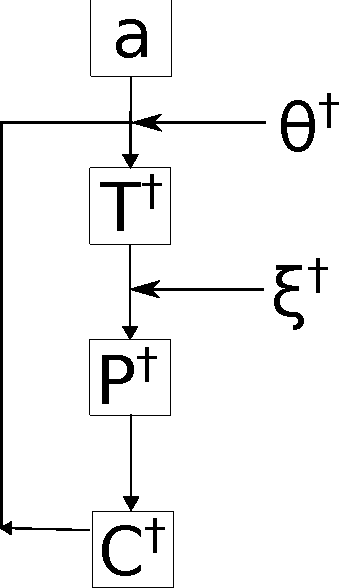
\includegraphics{chapters/adjoint_random_walk_process_derivation/random_walk_process.pdf}}
    \end{center}
  \caption{\textbf{Monte Carlo random walk process for adjoint radiation.}
    \textit{A particle state is first sampled from the adjoint source 
      distribution. The next collision point is sampled from the adjoint 
      transport kernel $T^{\dagger}$. Next, the adjoint particle weight is
      multiplied by the adjoint weight factor $P^{\dagger}$. Finally, the new 
      energy and direction is sampled from the adjoint collision kernel. This
      process continues until Russian roulette forces the random walk to
      terminate. This process allows both the adjoint emission density and 
      the adjoint collision density to be estimated.}}
  \label{fig:combined_adj_random_walk_process}
\end{figure}

\section{Estimating Responses}
Due to the way that the adjoint transport equation is constructed, the inner
product of the adjoint flux $\varphi^{\dagger}(\vec{r},E,\hat{\Omega})$ and the
source $S(\vec{r},E,\hat{\Omega})$ will result in the same value as the inner 
product of the flux $\varphi(\vec{r},E,\hat{\Omega})$ and the response
function $a(\vec{r},E,\hat{\Omega})$. Because it is not ideal to estimate the
adjoint flux directly using a Monte Carlo random walk process, equivalent
inner products must be constructed that are either in terms of the adjoint
collision density or the adjoint emission density:
\begin{align}
  I & = \int\int\int S(\vec{r},E,\hat{\Omega})\varphi^{\dagger}(\vec{r},E,\hat{\Omega})
  dV dE d\hat{\Omega} \\ 
  & = \int\int\int U(\vec{r},E,\hat{\Omega})\xi^{\dagger}(\vec{r},E,\hat{\Omega})
  dV dE d\hat{\Omega} \\
  & = \int\int\int V(\vec{r},E,\hat{\Omega})
  \theta^{\dagger}(\vec{r},E,\hat{\Omega}).
  dV dE d\hat{\Omega}
  \label{eq:adj_emission_ip}
\end{align}
Based on the relationship between the adjoint collision density and the
adjoint flux, $U(\vec{r},E,\hat{\Omega})$ must be defined as
\begin{equation}
  U(\vec{r},E,\hat{\Omega}) = \frac{S(\vec{r},E,\hat{\Omega})}
                                   {\Sigma_T(\vec{r},E,\hat{\Omega})}.
\end{equation}
Similarly, the function $V(\vec{r},E,\hat{\Omega})$ must be defined as
\begin{equation}
  V(\vec{r},E,\hat{\Omega}) = \int \frac{S(\vec{r}^{'},E,\hat{\Omega})}
  {\Sigma_T(\vec{r}^{'},E,\hat{\Omega})} 
  T^{\dagger}(\vec{r} \to \vec{r}^{'},E,\hat{\Omega}) dV^{'}.
\end{equation}
Clearly, the function $U(\vec{r},E,\hat{\Omega})$ will be easier to evaluate
than the function $V(\vec{r},E,\hat{\Omega})$. Using either of the estimators
that were described in chapter \ref{ch:mc_methods} or the track-length 
estimator that was described in chapter \ref{ch:particle_transport} and the 
combined random walk process that was outlined in the previous section, an 
estimate for the value I can be obtained. 

\section{Chapter Summary}
Several points from this chapter must be emphasized before moving on:
\begin{itemize}
  \item The dual emission density FIESK and the dual collision density FIESK
    describe ``flux-like'' quantities and should be avoided, based one of the 
    main points from the previous chapter.
  \item The material response calculated from the inner product of the flux
    and the material response function can also be calculated from the inner
    product of the source function and a new quantity called the adjoint flux,
    which is described by the adjoint transport equation.
  \item The adjoint transport equation can be constructed from the transport
    equation using a similar procedure to the one that was outlined in 
    chapter \ref{ch:mc_methods} for deriving a dual FIESK from a FIESK.
  \item By performing a set of manipulations similar to the ones outlined in
    the previous chapter, the integro-differential adjoint transport equation
    can be converted to a FIESK that describes the adjoint flux, the adjoint
    emission density or the adjoint collision density of a system.
  \item The adjoint emission density FIESK and the adjoint collision density
    FIESK are not equivalent to the dual emission density FIESK or the dual
    collision density FIESK respectively. However, they are related by a
    function $\Sigma^{*}(\vec{r},E)$, which has some specific properties. This 
    relationship becomes useful in the context of coupled adjoint neutron
    and adjoint photon transport.
  \item The state transition kernels that appear in the adjoint emission
    density FIESK and the adjoint collision density FIESK can be decomposed
    into two kernels and a weight factor: the adjoint collision kernel, which
    describes the movement of adjoint particles through energy and direction,
    the adjoint transport kernel, which describes the movement of adjoint 
    particles through space, and the adjoint weight factor.
  \item The adjoint weight factor comes about from the construction of the
    adjoint collision kernel and the adjoint transport kernel, both of which
    are normalized to unity. The adjoint collision kernel is constructed
    with the total macroscopic adjoint cross section while the adjoint
    transport kernel is constructed with the total macroscopic cross section.
    These cross sections are in general not equal, which gives rise to the
    adjoint weight factor.
  \item The adjoint collision kernel can be decomposed into its constituent
    adjoint reactions so that each reaction can be modeled explicitly.
  \item Every adjoint reaction must be constructed from a corresponding
    forward reaction using the following equations:
    \begin{equation*}
      \sigma^{\dagger}(E^{'}) = \int\int \sigma(E)c(E)
      p(E \to E^{'}, \hat{\Omega} \to \hat{\Omega}^{'}) dE d\hat{\Omega}
    \end{equation*}
    \begin{equation*}
      p^{\dagger}(E^{'} \to E, \hat{\Omega}^{'} \to \hat{\Omega}) = 
      \frac{\sigma(E)c(E)p(E \to E^{'}, \hat{\Omega} \to \hat{\Omega}^{'})}
      {\sigma^{\dagger}(E^{'})}
    \end{equation*}
  \item There are no adjoint absorption reactions or multiplication reactions.
    This is a result of the normalization of the adjoint collision kernel and
    the definition of the adjoint cross section.   
  \item Due to the similarity between the adjoint emission density FIESK and
    the adjoint collision density FIESK, solutions to both FIESKs can be 
    estimated using the same random walk process.
\end{itemize}

While all of the above points are important take-aways from this chapter, the
most interesting are certainly the existence of the adjoint weight factor, 
the definition of the adjoint cross section and the nonexistence of adjoint
absorption or multiplication reactions. 
